\documentclass{beamer}
\usepackage{smarky-theme}
\usepackage{tikz}
\usepackage{amsmath}
\usepackage{hyperref}


\title{Example}
\subtitle{Hello, World}
\author{Sam A. Markelon}
\date{September 2, 2025}

\begin{document}

% Title slide
\begin{frame}[plain]
  \centering
  \vspace*{2cm}
  {\usebeamercolor[fg]{title}\usebeamerfont{title}\LARGE \inserttitle\par}
  \vspace{0.5em}
  {\usebeamercolor[fg]{subtitle}\usebeamerfont{subtitle}\Large \insertsubtitle\par}
  \vspace{1em}
  {\usebeamercolor[fg]{author}\usebeamerfont{author}\large \insertauthor\par}
  \vspace{0.5em}
  {\usebeamercolor[fg]{date}\normalsize \insertdate\par}
\end{frame}

% Starting Slide
\begin{frame}{smarky-theme}
\begin{itemize}
  \item The beamer theme is the same as smarky-colors.
  \item Everything here is written in navy on a warm off-white background, with \emph{golden accents} where needed.
  \item Visit: \url{https://smarky7cd.github.io}. 
\end{itemize}
\end{frame}

% Block example
\begin{frame}{Key Takeaway}
\begin{block}{Block Example}
This is an example of a block.
\end{block}
\end{frame}

% Bayes' Law Slide
\begin{frame}{Bayes' Law}
\[
P(A \mid B) = \frac{P(B \mid A) \cdot P(A)}{P(B)}
\]
\pause
\begin{block}{Interpretation}
Bayes’ Law allows us to update our beliefs about \(A\) after observing \(B\), assuming we know:
\begin{itemize}
  \item \(P(A)\): prior belief
  \item \(P(B \mid A)\): likelihood
  \item \(P(B)\): evidence
\end{itemize}
\end{block}
\end{frame}

% TikZ Tree Slide
\begin{frame}{Binary Search Tree}
\centering
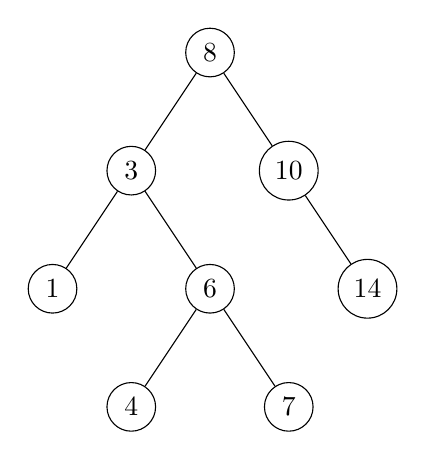
\begin{tikzpicture}[sibling distance=20mm, every node/.style={draw,circle}]
  \node {8}
    child { node {3}
      child { node {1} }
      child { node {6}
        child { node {4} }
        child { node {7} }
      }
    }
    child { node {10}
      child[missing]
      child { node {14}
      }
    };
\end{tikzpicture}
\end{frame}

% Final slide
\begin{frame}{Thanks!}
  Questions? Discussion welcome.
\end{frame}

\end{document}